\documentclass[11pt,a4paper]{article}
\usepackage[margin=2.3cm]{geometry}
\usepackage[T1]{fontenc}
\usepackage{lmodern}
\usepackage{amsmath,amssymb}
\usepackage{graphicx}
\usepackage{xcolor}
\usepackage{listings}
\usepackage{fancyhdr}
\usepackage{titlesec}
\usepackage{enumitem}
\usepackage{booktabs}
\usepackage{array}
\usepackage{longtable}
\usepackage{tcolorbox}
\usepackage[htt]{hyphenat}
\usepackage{xurl}
\usepackage[hidelinks]{hyperref}
\usepackage{float}

\graphicspath{{../../assets/}}

% ---------- running header (same as last year) ----------
\pagestyle{fancy}
\fancyhf{}
\fancyhead[L]{\textit{WiDS 2026}}
\fancyhead[R]{\textit{Re-Mind}}
\fancyfoot[C]{\thepage}
\renewcommand{\headrulewidth}{0.4pt}

% ---------- big centred sections with a cheeky subtitle ----------
\titleformat{\section}{\normalfont\Large\bfseries\filcenter}{\thesection}{1em}{}
\titlespacing*{\section}{0pt}{0.4em}{0.5em}
\usepackage{needspace}
\usepackage{tocloft}
\setlength{\cftbeforesecskip}{3pt}
\newcommand{\bigsection}[2]{%
  \par\Needspace{12\baselineskip}\bigskip\noindent\rule{\linewidth}{0.4pt}\par
  \vspace{-0.4em}%
  \section{#1}%
  {\centering\textbf{#2}\par}%
  \vspace{0.3em}\noindent\rule{\linewidth}{0.4pt}\par\medskip}

\setlist[itemize]{leftmargin=1.4em, itemsep=0.35em}

% ---------- week banner ----------
\newcommand{\weekbanner}[3]{%
  \clearpage
  \begin{center}
  {\small\scshape Winter in Data Science \,·\, Re-Mind 2.0}\\[0.6em]
  {\Huge\bfseries #1}\\[0.4em]
  {\Large #2}\\[0.8em]
  \begin{minipage}{0.82\linewidth}\centering\itshape #3\end{minipage}
  \end{center}
  \vspace{0.4em}}

% ---------- code ----------
\lstset{
  language=Python,
  basicstyle=\ttfamily\small,
  keywordstyle=\bfseries,
  commentstyle=\itshape\color{black!60},
  stringstyle=\color{black!80},
  numbers=left, numberstyle=\tiny, numbersep=6pt,
  columns=fullflexible, keepspaces=true,
  breaklines=true, showstringspaces=false,
  frame=none, xleftmargin=1.5em,
  aboveskip=0.6em, belowskip=0.6em,
  literate={→}{$\rightarrow$}1 {—}{---}1
}
\lstdefinestyle{shell}{language=bash, numbers=none, xleftmargin=1.5em}

% ---------- boxes ----------
\newtcolorbox{task}[1]{colback=white, colframe=black, boxrule=0.5pt, arc=0pt,
  left=6pt, right=6pt, top=4pt, bottom=4pt, title={\textbf{#1}}, coltitle=black, colbacktitle=black!8}
\newtcolorbox{note}{colback=black!4, colframe=black!4, arc=0pt, left=6pt, right=6pt, top=4pt, bottom=4pt}

% function-table rows like last year
\newcommand{\fnrow}[4]{\textbf{Function / Class} & \textbf{Description}\\ \texttt{#1} & #2\\ \textbf{Syntax Example} & \textbf{Use Case}\\ \texttt{#3} & #4\\ \hline}


\begin{document}

% ======================= TITLE =======================
\begin{center}
{\LARGE\bfseries Re-mind 2.0 : An agentic AI tutor that\\[0.2em] learns when you'll forget}\\[0.6em]
{\Large\bfseries The Complete Handbook --- Weeks 1 to 5}\\[1.2em]
{\large Muhammed Sufiyan \quad \& \quad Anshuman Gupta}\\[0.3em]
\textit{Winter in Data Science Projects \,·\, WiDS 6.0 \,·\, Analytics Club, IIT Bombay}
\end{center}

\noindent\rule{\linewidth}{0.4pt}
\paragraph{Abstract}
Last year we built Re-Mind: a chatbot that saved your questions and quizzed you on them every five
questions or every ten minutes. It worked, but the \emph{rules} were ours --- the bot never got better at
deciding \emph{when} to test you. This year we amp it up. Over five weeks you will build the tutor step by step:
first an LLM chatbot with memory (Week 1), then an \emph{agentic} tutor that quizzes, grades and teaches
Socratically on its own (Week 2). Then we learn Reinforcement Learning from scratch (Week 3), use it to
build a scheduler that learns the best gap before each review on thousands of simulated students (Week 4),
and finally plug that agent into the live tutor so that every quiz grade becomes a reward that keeps it learning
while you study (Week 5). Each week has reading material (this handbook), runnable notebooks and code in
the GitHub repo, a weekly meet, and an assignment. In case you do not understand something here, ask on the
group or refer to other sources as well. All the best and happy learning!
\par\noindent\rule{\linewidth}{0.4pt}

\tableofcontents
\clearpage

% ======================= ROADMAP =======================
\bigsection{How this project works}{read this once, then keep it open in a tab.}

\subsection{The 5-week roadmap}
\begin{center}
\renewcommand{\arraystretch}{1.25}
\begin{tabular}{@{}p{1.1cm}p{4.1cm}p{5.2cm}p{4.1cm}@{}}
\toprule
\textbf{Week} & \textbf{Theme} & \textbf{You build} & \textbf{Deliverable}\\
\midrule
1 & Foundations \newline\textit{(self-paced)} & Gemini chatbot that stores every chat in JSON & \texttt{app.py}\\
2 & The agentic chatbot & context, autonomous quizzes, JSON grader, Socratic mode & \textbf{Mid-term}: three bots\\
3 & RL from scratch & bandits, Q-learning in a gridworld & 2 notebooks\\
4 & Spaced repetition: rules vs RL & simulated student, Leitner, RL scheduler, reward hacking & notebooks + 1-page comparison\\
5 & RL inside the live tutor & grade $\rightarrow$ reward $\rightarrow$ online learning; demo; report & \textbf{End-term}\\
\bottomrule
\end{tabular}
\end{center}

\subsection{Logistics}
\begin{itemize}
  \item \textbf{Time:} about 7 hours a week. Every week = reading (this handbook) $\rightarrow$ hands-on notebook
        $\rightarrow$ build (assignment) $\rightarrow$ weekly meet (45--60 min).
  \item \textbf{Week 1 is self-paced.} We (the mentors) are busy with placements at the start. Everything you need
        for Week 1 is in this handbook and the repo; post doubts on the group and we'll catch up.
  \item \textbf{Repo:} \url{https://github.com/suff-yan/REMIND} --- every week has its own folder. The \texttt{remind/}
        package is our reference implementation: read it, import it, extend it.
  \item \textbf{AI tools are allowed}, but you must understand every line you submit: the final report is checked
        by the Analytics conveners.
\end{itemize}

\subsection{The big picture}
\begin{note}
\textbf{Re-Mind's loop.} You ask a question $\rightarrow$ Gemini answers $\rightarrow$ the tutor stores the
\emph{concept} you learned $\rightarrow$ an RL agent decides how many days to wait before quizzing you
$\rightarrow$ when it is due, the tutor interrupts you with a recall check $\rightarrow$ Gemini grades your answer
$\rightarrow$ the grade becomes a \emph{reward} that teaches the agent $\rightarrow$ repeat.
\end{note}
Weeks 1--2 build the left half of this loop (LLM + memory + autonomy). Weeks 3--4 build the right half (RL).
Week 5 closes the loop.

% ======================= WEEK 1 =======================
\weekbanner{Week 1}{Foundations}{From ``I know basic Python'' to ``my code talks to an LLM and remembers things''.
Self-paced --- take your time with the setup, it is the part everyone gets stuck on.}

\bigsection{Setting up your machine}{boring, but do it once and do it right.}

\subsection{Virtual environment and dependencies}
\begin{itemize}
  \item Install Python 3.11+ and VS Code. On Windows, preferably use WSL.
  \item Clone the repo and go inside it:
\begin{lstlisting}[style=shell]
git clone https://github.com/suff-yan/REMIND.git
cd REMIND
\end{lstlisting}
  \item Create and activate a virtual environment --- a private box of packages for this project only:
\begin{lstlisting}[style=shell]
python -m venv venv
source venv/bin/activate        # you should now see (venv) in the prompt
pip install -r requirements.txt
\end{lstlisting}
  \item Open the folder in VS Code with \texttt{code .} and select the \texttt{venv} interpreter.
\end{itemize}

\subsection{The API key, kept secret}
\begin{itemize}
  \item Get a free key from Google AI Studio (\url{https://aistudio.google.com/apikey}).
  \item Copy \texttt{.env.example} to \texttt{.env} and paste your key. \texttt{.env} is in \texttt{.gitignore} so it
        never reaches GitHub.
\begin{lstlisting}[style=shell]
GEMINI_API_KEY=your-key-here
GEMINI_MODEL=gemini-3.1-flash-lite
REMIND_DAY_SECONDS=60
\end{lstlisting}
  \item Run \texttt{python week1\_foundations/examples/hello\_gemini.py}. It lists the models your key can use and
        makes your first call. \textbf{Model names change every few months} (last year it was
        \texttt{gemini-2.5-flash-lite}) --- if a model name errors, pick a \emph{flash} or \emph{flash-lite} model from
        that list and put it in \texttt{.env}.
\end{itemize}

\bigsection{Application Programming Interface}{the core concept of this project and will be useful for a lot of interviews :)}

\subsection{What is an API ?}
\begin{itemize}
  \item The AI model you use --- Gemini --- is incredibly complex: billions of parameters running on powerful servers.
        As a programmer you don't need to know how it works inside. You talk to it through an \textbf{API}: a simple
        doorway into a giant system. You pass instructions through the door, and the result comes back.
  \item A helpful analogy is a restaurant. Gemini is the kitchen --- expert chefs, tools and ingredients you
        cannot access directly. The API is the waiter. You give a clear request (``create a quiz question about
        Newton's laws''), the waiter takes it to the kitchen and comes back with a neatly prepared response.
        This is exactly what happens when your code calls \texttt{client.models.generate\_content(...)}.
  \item The beauty of an API is that it hides the messy details. You are not controlling \emph{how} the AI thinks;
        you are controlling \emph{how you ask} it to think. In Re-Mind, the agent wraps your messages into
        structured prompts (``answer this'', ``write a quiz'', ``grade this answer'') and uses the replies to decide
        what to do next.
\end{itemize}

\subsection{What is an API key ?}
\begin{itemize}
  \item Millions of people use the same AI. Gemini needs to know \emph{who} is making a request and how much they
        are allowed to use. That identity card is the \textbf{API key}: a long secret string, like a password or a
        library card.
  \item Because it is as powerful as a password, it must stay secret --- never hard-code it in your script.
        Store it in \texttt{.env} and read it with \texttt{os.getenv()}. Keep your credit card in your wallet,
        not printed on your T-shirt.
  \item The free tier has rate limits. If you hit them you'll see a \texttt{429 / RESOURCE\_EXHAUSTED} error:
        wait a minute, or switch to a \emph{lite} model.
\end{itemize}

\bigsection{Python Knowledge}{some extra libraries exclusive to this project.}

\subsection{The \texttt{os} module and \texttt{dotenv}}
\begin{lstlisting}
import os
from dotenv import load_dotenv
load_dotenv()                                  # reads .env into environment variables
api_key = os.getenv("GEMINI_API_KEY")          # None if missing
\end{lstlisting}
Other useful functions: \texttt{os.path.exists(p)}, \texttt{os.path.join(a, b)}, \texttt{os.listdir()} and \texttt{os.makedirs(p, exist\_ok=True)}.

\subsection{Google GenAI SDK: talking to Gemini}
\begin{lstlisting}
from google import genai
from google.genai import types

client = genai.Client(api_key=api_key)
MODEL = os.getenv("GEMINI_MODEL", "gemini-3.1-flash-lite")

response = client.models.generate_content(model=MODEL, contents="Explain gravity simply.")
print(response.text)
\end{lstlisting}
\begin{note}
Last year's handbook showed \texttt{genai.configure(...)} and \texttt{genai.GenerativeModel(...)}. That is the
\emph{old} \texttt{google-generativeai} library, now deprecated. This year we only use the new \texttt{google-genai}
SDK with \texttt{genai.Client}. If you copy code from the internet, check which one it uses!
\end{note}

\subsection{Error handling: how to prevent crashes}
AI services sometimes fail: too many requests, no quota, wrong model name, bad internet. Instead of crashing, catch errors:
\begin{lstlisting}
try:
    response = client.models.generate_content(model=MODEL, contents=prompt)
    reply = response.text
except Exception as e:
    reply = f"API error: {e}"          # show it in the UI, don't crash
\end{lstlisting}

\subsection{Storing chats locally --- the \texttt{json} module}
While a program runs, its data lives in memory and is lost when it stops. The \texttt{json} module is a bridge to
long-term memory on disk: \texttt{json.dump()} writes Python dicts and lists to a file, \texttt{json.load()} brings
them back. JSON is human-readable, so you can open the file and watch your bot's memory grow.
Work through \texttt{week1\_foundations/02\_json\_and\_datetime.ipynb}. The one pattern you'll use everywhere:
\begin{lstlisting}
def load_data():
    if not os.path.exists(DATA_FILE):
        return {"interactions": []}
    try:
        with open(DATA_FILE) as f:
            return json.load(f)
    except json.JSONDecodeError:         # empty or corrupted file
        return {"interactions": []}
\end{lstlisting}

\subsection{Getting the time --- the \texttt{datetime} module}
Spaced repetition is all about \emph{when}. JSON has no date type, so we store ISO strings and convert back to do arithmetic:
\begin{lstlisting}
from datetime import datetime, timedelta
stamp = datetime.now().isoformat()                       # '2026-12-14T22:50:37.748526'
elapsed = datetime.now() - datetime.fromisoformat(stamp)
is_due = elapsed >= timedelta(minutes=10)
\end{lstlisting}
\textbf{Pro tip:} write functions like \texttt{is\_due(item, now)} that take \texttt{now} as an argument. Then you can
test your scheduler with a fake clock instead of waiting for days.

\bigsection{Making your first chatbot}{We will build a simple LLM clone this week.}

\subsection{How Streamlit thinks}
Streamlit turns a Python script into a web app. The one thing to understand: \textbf{the whole script re-runs from
top to bottom on every interaction}. Normal variables are reset every time; anything you want to keep across
reruns goes into \texttt{st.session\_state}.

\subsection{The code, block by block}
The full file is \nolinkurl{week1_foundations/examples/app.py}. Run it with:
\begin{lstlisting}[style=shell]
streamlit run week1_foundations/examples/app.py
\end{lstlisting}
\begin{lstlisting}
st.title("Gemini clone with saved history")
if "chat" not in st.session_state:            # survives reruns
    st.session_state.chat = []

for msg in st.session_state.chat:             # redraw the conversation
    with st.chat_message(msg["role"]):
        st.markdown(msg["content"])

if user_input := st.chat_input("Ask anything..."):
    st.session_state.chat.append({"role": "user", "content": user_input})
    response = client.models.generate_content(
        model=MODEL,
        contents=[types.Content(role="user", parts=[types.Part.from_text(text=user_input)])])
    reply = response.text
    st.session_state.chat.append({"role": "assistant", "content": reply})
    save_interaction(user_input, reply)       # load -> append -> save to JSON
\end{lstlisting}
\begin{itemize}
  \item \texttt{st.session\_state.chat} holds the conversation for this browser tab; the JSON file holds it forever.
  \item The \texttt{:=} (walrus) operator assigns and checks in one go: ``if the user typed something, call it \texttt{user\_input}''.
  \item \texttt{save\_interaction} stores \texttt{\{query, response, time\}} --- the raw material for every quiz later.
\end{itemize}

\subsection{Cheatsheets}
\begin{center}
\small
\begin{tabular}{|>{\raggedright\arraybackslash}p{5.6cm}|>{\raggedright\arraybackslash}p{8.2cm}|}
\hline
\multicolumn{2}{|c|}{\textbf{Google Gemini (\texttt{google-genai}) functions used}}\\ \hline
\fnrow{genai.Client()}{Connects to Gemini with your API key.}{genai.Client(api\_key=KEY)}{Created once at the top of the app.}
\fnrow{client.models.generate\_content()}{Sends prompt(s) and returns the reply.}{generate\_content(model, contents, config)}{Answers, quizzes, grades --- everything.}
\fnrow{client.models.list()}{Lists models your key can use.}{for m in client.models.list(): ...}{Find a valid model name.}
\fnrow{types.Content()}{One message with a role (\texttt{user} / \texttt{model}).}{types.Content(role="user", parts=[...])}{Sending conversation history (Week 2).}
\fnrow{types.Part.from\_text()}{A text piece inside a message.}{types.Part.from\_text(text="Hi")}{Wrapping plain text for Gemini.}
\fnrow{types.GenerateContentConfig()}{Options: system instruction, temperature, JSON output.}{GenerateContentConfig(response\_mime\_type= "application/json")}{Structured grades (Week 2), Socratic mode.}
\end{tabular}
\end{center}

\begin{center}
\small
\begin{tabular}{|>{\raggedright\arraybackslash}p{5.6cm}|>{\raggedright\arraybackslash}p{8.2cm}|}
\hline
\multicolumn{2}{|c|}{\textbf{Streamlit functions used}}\\ \hline
\fnrow{st.title() / st.caption()}{Page heading and small text.}{st.title("Re-Mind")}{Top of the app.}
\fnrow{st.session\_state}{Variables that survive reruns.}{st.session\_state.chat}{Chat history, pending quiz.}
\fnrow{st.chat\_message()}{A chat bubble for a role.}{with st.chat\_message("user"):}{Drawing the conversation.}
\fnrow{st.chat\_input()}{Chat box; returns text or None.}{if q := st.chat\_input("Ask"):}{Reading the user's message.}
\fnrow{st.sidebar / st.button()}{Side panel and buttons.}{if st.sidebar.button("Quiz me"):}{Controls and history.}
\fnrow{st.rerun()}{Re-run the script immediately.}{st.rerun()}{Refresh after updating state.}
\end{tabular}
\end{center}

\begin{task}{Week 1 assignment}
Write \textbf{your own} \texttt{app.py}: a chatbot that saves \texttt{\{query, response, time\}} to JSON and shows the
last 10 saved queries in the sidebar. Bonus: a ``Clear history'' button and a counter of questions asked today.
Submit a GitHub/Drive link and a screenshot of your JSON file.
\end{task}

% ======================= WEEK 2 =======================
\weekbanner{Week 2}{The Agentic Chatbot}{The bot stops being passive: it remembers the conversation, decides by itself
when to quiz you, grades you in a format code can use, and can teach Socratically.}

\bigsection{But what even is agentic AI ?}{sounds really cool and tough but actually is fairly simple.}

\subsection{Definition}
\begin{itemize}
  \item Agentic AI refers to AI systems that don't just respond to inputs, but also take initiative, make decisions
        and manage their own workflow. A normal model answers your question and waits. An agentic system can store
        information, plan, choose tools, check its own work, and sometimes act without being explicitly asked.
  \item The key idea is \textbf{agency} --- the ability to decide the next action. An agent typically has four parts:
        an LLM as the ``brain'', \textbf{memory}, \textbf{tools} or APIs it can call, and a \textbf{decision}
        mechanism. They run in a loop: \emph{perceive $\rightarrow$ decide $\rightarrow$ act $\rightarrow$ remember}.
\end{itemize}

\subsection{Agentic AI v/s AI agents}
Agentic AI is the \emph{idea} --- autonomy and initiative. An AI agent is the \emph{thing} built using that idea:
a concrete program with a model, memory, rules and a loop. Re-Mind is an AI agent.

\subsection{OK, but how is this related to the project ?}
\begin{center}
\begin{tabular}{@{}lll@{}}
\toprule
\textbf{Agent part} & \textbf{Last year (WiDS 5.0)} & \textbf{This year}\\
\midrule
Brain & Gemini & Gemini\\
Memory & JSON of queries & JSON of \emph{concepts} with review history\\
Tools & quiz + grade prompts & quiz, JSON grader, concept extractor\\
Decision: \emph{when to quiz?} & fixed rule (5 questions / 10 min) & \textbf{learned by RL} (Weeks 3--5)\\
\bottomrule
\end{tabular}
\end{center}
That last row is the whole point of this year's project. This week we build the agent with a hand-written decision rule;
by Week 5 that rule is replaced by a learned one.

\bigsection{Context saving for a conversation}{so the bot doesn't forget what you said 10 seconds ago.}
\begin{itemize}
  \item The Week 1 bot sends \emph{one} message at a time, so it has no idea what you said before. Ask it
        ``what is entropy?'' then ``give an example'' --- it won't know an example \emph{of what}.
  \item Fix: send the conversation. Gemini calls the bot's role \texttt{model} (not \texttt{assistant}):
\begin{lstlisting}
def to_gemini(messages):
    return [types.Content(role="user" if m["role"] == "user" else "model",
                          parts=[types.Part.from_text(text=m["content"])])
            for m in messages]

resp = client.models.generate_content(model=MODEL, contents=to_gemini(messages[-20:]))
\end{lstlisting}
  \item \texttt{messages[-20:]} keeps only the last 20 messages --- every token you send costs quota and time.
        See \texttt{week2\_agentic\_chatbot/examples/context\_chat.py}.
\end{itemize}

\bigsection{Making the bot act on its own}{the first taste of agency: nobody pressed ``quiz me''.}

\subsection{Trigger 1: a counter}
Keep \texttt{st.session\_state.recent\_questions}. After each answer, append the question; when there are $N=5$,
pick one with \texttt{random.choice}, ask Gemini for a quiz question on it, store it as \texttt{pending\_quiz}, and
show it. The next message from the user is treated as the answer.

\subsection{Trigger 2: a clock}
Store \texttt{asked\_at} for each question. At the top of every rerun, check whether any question is older than
10 minutes and not yet quizzed. If so --- quiz. The bot interrupts \emph{you}.

\subsection{Pending-quiz pattern}
\begin{lstlisting}
if user := st.chat_input():
    if st.session_state.pending_quiz:        # this message is an ANSWER
        grade, feedback = grade_answer(st.session_state.pending_quiz, user)
        st.session_state.pending_quiz = None
    else:                                    # this message is a QUESTION
        reply = answer(user)
        maybe_start_quiz()                   # counter / clock decides
\end{lstlisting}

\bigsection{Grading with structured output}{a grade your code can actually use.}
Last year the examiner prompt returned text starting with ``Correct:'' or ``Incorrect:''. Fine for humans, painful
for code. This year we ask for \textbf{JSON}:
\begin{lstlisting}
resp = client.models.generate_content(
    model=MODEL,
    contents=GRADE_PROMPT.format(fact=fact, question=q, answer=a),
    config=types.GenerateContentConfig(response_mime_type="application/json", temperature=0))
data = json.loads(resp.text)           # {"grade": 2, "feedback": "Spot on."}
\end{lstlisting}
\begin{itemize}
  \item Grades: \textbf{0} = forgot/wrong, \textbf{1} = partly right/hesitant, \textbf{2} = clearly correct.
        These three numbers become the RL agent's observations and rewards in Week 5 --- remember them!
  \item \texttt{temperature=0} makes the grader as deterministic as possible.
  \item Always wrap \texttt{json.loads} in \texttt{try/except}; LLMs occasionally return something odd.
\end{itemize}

\bigsection{Socratic Mode}{learning through a dialogue.}
\subsection{About the method}
The Socratic way of studying is learning by questioning instead of passively absorbing. Each question forces
clarity; each vague answer shows you exactly where your understanding is shallow. Combined with Feynman's
insistence on simplicity, it builds understanding rather than recognition.

\subsection{System instructions}
Last year we pasted the Socratic rules into the user's message, and the bot sometimes wrote a fake conversation
with itself. The cleaner way is a \textbf{system instruction} --- a personality that holds for the whole chat:
\begin{lstlisting}
SOCRATIC = """You are a Socratic tutor. Guide the student with short questions instead of
answers. Ask ONE question at a time and stop - never write the student's reply yourself.
If the student is stuck after two attempts, give a small hint."""

config = types.GenerateContentConfig(system_instruction=SOCRATIC, temperature=0.7)
\end{lstlisting}
See \texttt{examples/socratic\_bot.py}. If the bot still answers directly, make the rules more explicit and test again.

\bigsection{Mid-Term submission}{please dont take an year to do it :P}
\begin{task}{Mid-term (due end of Week 2)}
\begin{enumerate}[leftmargin=1.4em]
  \item \textbf{\texttt{counterbot.py}} --- counts questions; after 5 it quizzes you on a random one of them
        \emph{without being asked}, then resets. Start from \texttt{starter/counterbot.py}.
  \item \textbf{\texttt{timebot.py}} --- stores the time of each question and quizzes you on any question older than
        10 minutes. Start from \texttt{starter/timebot.py} (use 1 minute while testing).
  \item \textbf{\texttt{gradebot.py}} --- either bot + the JSON grader: every quiz answer gets
        \texttt{\{grade, feedback\}} and the grade is saved in the JSON memory.
\end{enumerate}
Put the files in a Drive folder or GitHub repo and submit the link in the form. Submission is mandatory --- reach out
if you're stuck.
\end{task}

% ======================= WEEK 3 =======================
\weekbanner{Week 3}{Reinforcement Learning from Scratch}{No ML background needed. By the end of this week you will
have implemented the algorithm that schedules your quizzes in Week 5.}

\bigsection{What is Reinforcement Learning ?}{learning by trial, error, and a number called reward.}
\subsection{The vocabulary}
\begin{itemize}
  \item \textbf{Agent} --- the decision maker (our scheduler). \textbf{Environment} --- everything else (the student).
  \item \textbf{State} $s$ --- what the agent knows right now. \textbf{Action} $a$ --- what it can do.
  \item \textbf{Reward} $r$ --- a number saying how good the last step was. The agent's only goal is to collect as
        much reward as possible over time.
  \item \textbf{Policy} $\pi(s)$ --- the agent's strategy: which action to take in each state.
\end{itemize}
Supervised learning is told the right answer. RL is never told the right answer --- only how good its choice was,
often much later. That is why it needs to \emph{explore}.

\subsection{The agent--environment loop}
Every RL program you'll ever write has this shape (\texttt{remind/rl/qlearning.py}):
\begin{lstlisting}
state = env.reset()
while not done:
    action = agent.act(state)
    next_state, reward, done, info = env.step(action)
    agent.update(state, action, reward, next_state, done)
    state = next_state
\end{lstlisting}

\bigsection{Multi-armed bandits}{the simplest RL problem: one state, many choices.}
\subsection{The story}
Re-Mind can quiz you in 4 styles: MCQ, fill-in-the-blank, true/false, explain-in-your-own-words. Each style has an
unknown chance $p_k$ of really helping you remember. Every quiz is a pull of a slot-machine ``arm''. Which style should
the tutor use?

\subsection{Estimating values}
After $n$ pulls of arm $a$, estimate its value by the average reward. Incrementally:
\[ Q_{n+1}(a) = Q_n(a) + \frac{1}{n}\big(r - Q_n(a)\big) \]
\emph{New estimate = old estimate + step size $\times$ error.} Remember this shape --- Q-learning has exactly the same one.

\subsection{Exploration vs exploitation}
\begin{itemize}
  \item \textbf{Greedy:} always pick the arm that looks best. A trap --- if the best arm is unlucky early, it's never tried again.
  \item \textbf{$\varepsilon$-greedy:} with probability $\varepsilon$ pick a random arm, otherwise the best one.
  \item \textbf{UCB} (upper confidence bound): be optimistic about arms you haven't tried much,
        \[ a_t = \arg\max_a \; Q(a) + \sqrt{\frac{c \ln t}{N(a)}} . \]
\end{itemize}
\begin{figure}[H]\centering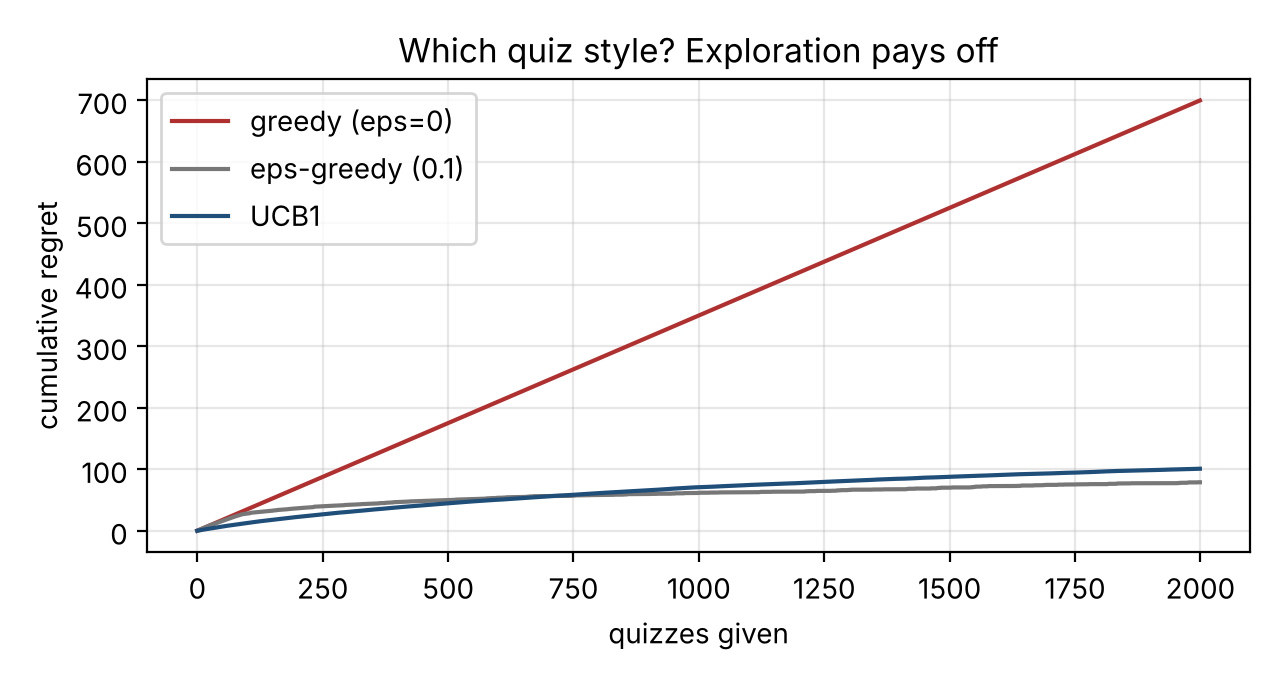
\includegraphics[width=0.78\linewidth]{bandit_regret.png}
\caption{Average over 50 runs. \emph{Regret} = reward lost vs always using the best arm. Greedy keeps losing; any exploration fixes it.}\end{figure}
Notebook: \texttt{week3\_rl\_foundations/01\_bandits.ipynb}.

\bigsection{MDPs and Q-learning}{when your actions change what happens next.}
\subsection{Markov Decision Processes}
Bandits have one state. Most problems have states that \emph{change because of your actions}: that is an MDP ---
states, actions, rewards, transitions, and a discount factor $\gamma$. The agent maximises the \textbf{return}
\[ G_t = r_{t+1} + \gamma r_{t+2} + \gamma^2 r_{t+3} + \dots \qquad (0 \le \gamma < 1). \]
$\gamma$ close to 1 = patient, cares about the far future; close to 0 = greedy for immediate reward.

\subsection{Q-values and the Q-learning update}
$Q(s,a)$ = expected return if we take action $a$ in state $s$ and act well afterwards. If we knew $Q$, acting would be easy:
$\pi(s) = \arg\max_a Q(s,a)$. Q-learning learns it from experience:
\[ Q(s,a) \leftarrow Q(s,a) + \alpha\Big[\underbrace{r + \gamma \max_{a'} Q(s',a')}_{\text{target}} - Q(s,a)\Big] \]
Same shape as the bandit running mean, but the target \emph{looks one step ahead}. The whole algorithm:
\begin{lstlisting}
def update(self, s, a, r, s_next, done):
    target = r if done else r + self.gamma * max(self.q[s_next])
    self.q[s][a] += self.alpha * (target - self.q[s][a])
\end{lstlisting}

\subsection{The study-room gridworld}
\begin{minipage}{0.52\linewidth}
Get from \textbf{S} to the exam hall \textbf{G} (+10) without picking up your phone \textbf{X} ($-5$, episode over).
Each step costs $-0.1$. After $\sim$400 episodes the agent finds a shortest safe path:
\begin{verbatim}
  learned policy      layout
     > > v <           S . . .
     ^ # v X           . # . X
     > > v v           . . . .
     X > > G           X . . G
\end{verbatim}
\end{minipage}\hfill
\begin{minipage}{0.45\linewidth}\centering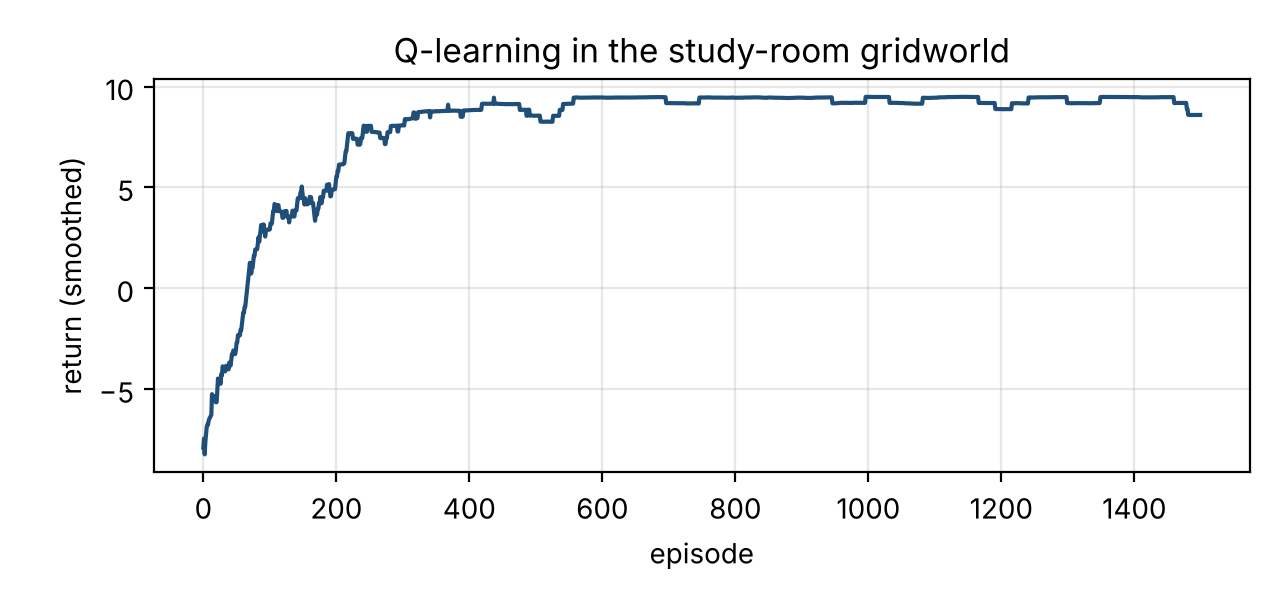
\includegraphics[width=\linewidth]{gridworld_curve.png}\end{minipage}

\medskip
Notebook: \texttt{week3\_rl\_foundations/02\_q\_learning\_gridworld.ipynb}.

\begin{task}{Week 3 assignment}
Answer the exercises at the end of both notebooks. Required: bandits 1, 2, 4 (decaying $\varepsilon$, close arms,
how the tutor could use a bandit) and gridworld 1, 2, 4 ($\gamma$ sweep, zero step cost, SARSA).
\end{task}

% ======================= WEEK 4 =======================
\weekbanner{Week 4}{Spaced Repetition: Rules vs RL}{We turn ``when should I quiz you?'' into an RL problem, build a
fake student to practise on, and try to beat the classic rule-based schedule.}

\bigsection{Spaced repetition}{A method to remember things.}
\subsection{yapping about why you should try out this method}
\begin{itemize}
  \item Imagine your brain is a leaky bucket. You pour knowledge in today and some of it immediately starts
        dripping out. Spaced repetition is pouring water back in right before it empties, again and again, until the
        bucket stops leaking so much.
  \item When you return to an idea after some time and successfully remember it, your brain gets a strong signal:
        ``this keeps coming back --- it must matter'', and reinforces it. Each time, forgetting slows down.
  \item The key trick is \textbf{timing}. Review too soon and your brain learns almost nothing new. Wait too long and
        you relearn from scratch. The sweet spot is when recall feels slightly uncomfortable. Forgetting is not the
        enemy --- forgetting is the teacher.
  \item Cramming writes on a foggy mirror. Spaced repetition writes on stone. Slower, more boring, but it lasts.
\end{itemize}

\subsection{fair enough, but how to decide when to revise ?}
\begin{itemize}
  \item \textbf{Fixed schedules} (review after 1, 3, 7 days\ldots) treat every fact the same.
  \item \textbf{Leitner boxes / levels} --- last year's ``level'' idea: right answer $\Rightarrow$ next box with a longer gap,
        wrong answer $\Rightarrow$ back to box 0.
  \item \textbf{Ease factors} (SM-2, used by Anki for decades) multiply the gap by a per-card ``ease''.
  \item \textbf{Forgetting-curve models} predict recall probability and schedule just before it drops below a target.
  \item \textbf{Stability/difficulty models} (FSRS) track how strong a memory is and learn their parameters from data.
  \item \textbf{This project:} instead of designing the rule, we let an RL agent \emph{learn} it.
\end{itemize}

\bigsection{A model of forgetting}{so the agent can practise on a million fake students before it meets you.}
\subsection{The forgetting curve}
\[ P(\text{recall after } t \text{ days}) = 0.9^{\,t/S} \]
\textbf{Stability} $S$ = how many days until recall drops to 90\%. Big $S$ = slow forgetting.
\begin{figure}[H]\centering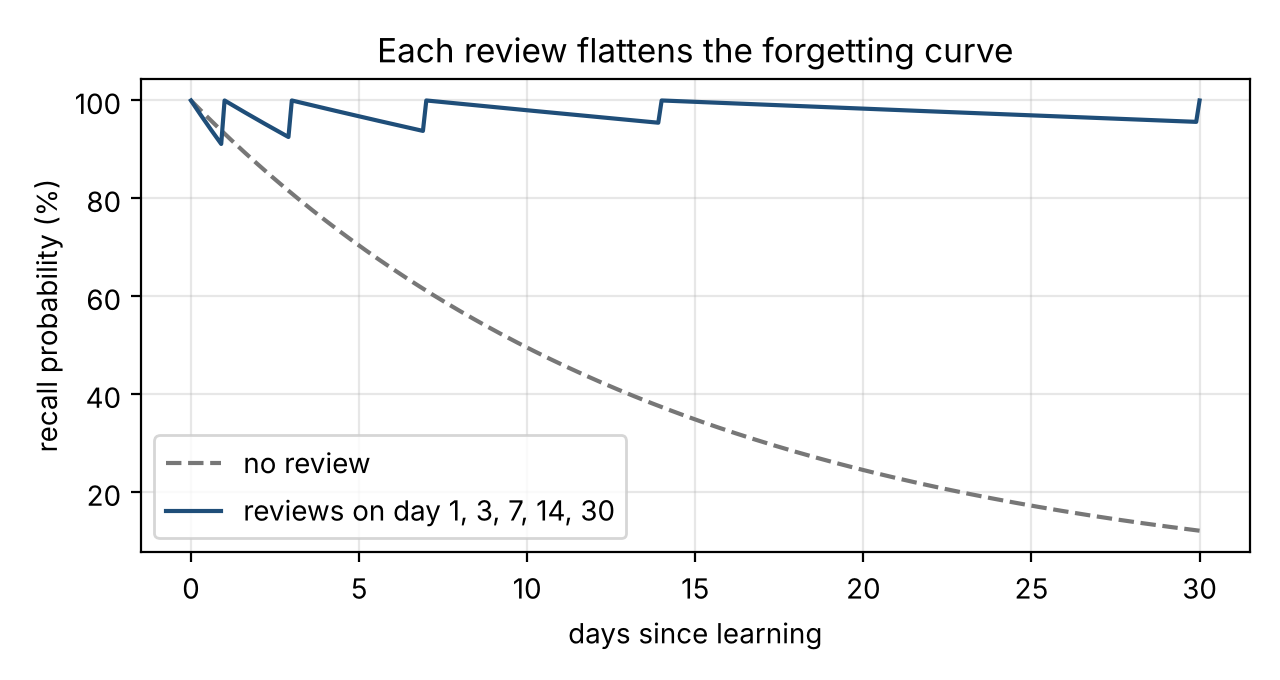
\includegraphics[width=0.78\linewidth]{forgetting_curve.png}
\caption{One simulated student. Without reviews recall decays; with reviews each dip is shallower and the gaps can grow.}\end{figure}

\subsection{The simulated student (\texttt{remind/memory\_model.py})}
Each concept has a hidden difficulty $d \in [0,1]$. When the student is quizzed after waiting $t$ days, they recall
with probability $p = 0.9^{t/S}$. Then:
\begin{itemize}
  \item \textbf{recalled:} $S \leftarrow S\cdot\big(1 + (2 - 1.8d)\,(1 + 2(1-p))\big)$ --- memory grows, and grows
        \emph{more} when recall was hard (low $p$). That's the ``slightly uncomfortable'' sweet spot in maths.
  \item \textbf{forgot:} $S \leftarrow 0.5\,S$.
  \item The student reports \emph{forgot / hard / easy} --- the same three grades Gemini gives in Week 5.
\end{itemize}
This is a simplified cousin of FSRS, not a scientific model of your brain. It is a sandbox.

\subsection{Leitner boxes, revisited}
Level = correct answers in a row; gaps per level: \textbf{1, 2, 4, 7, 14, 30 days}; wrong $\Rightarrow$ level 0.
It is a strong baseline --- but one ladder for every concept. On our simulator, Leitner keeps \textbf{99\%} recall on easy
concepts ($d=0.1$) but only \textbf{81\%} on hard ones ($d=0.9$). A fixed rule can't fit everyone.

\bigsection{Spaced repetition as an RL problem}{the heart of Re-Mind 2.0.}
\subsection{The MDP}
\begin{center}
\renewcommand{\arraystretch}{1.2}
\begin{tabular}{@{}p{3cm}p{11cm}@{}}
\toprule
\textbf{Episode} & one concept, from the day it is learned (day 0) to an exam on day 60\\
\textbf{State} & (correct-in-a-row streak $0..5$, last grade forgot/hard/easy) --- 18 states\\
\textbf{Action} & how many days to wait before the next quiz: 1, 2, 4, 7, 14 or 30\\
\textbf{Reward} & see below\\
\textbf{Environment} & the simulated student (\texttt{remind/env.py}, gym-style \texttt{reset}/\texttt{step})\\
\bottomrule
\end{tabular}
\end{center}
Notice the state contains only what a real tutor can observe --- never the hidden difficulty or stability.

\subsection{Designing the reward}
\[ r = \begin{cases} +\,\text{gap} - c & \text{if recalled} \\ -\,2\cdot\text{gap} - c & \text{if forgot} \end{cases} \qquad (c = 1 \text{ per review}) \]
\emph{If you waited 14 days and still remembered, you proved 14 days of memory.} Forgetting costs double, and every
review costs a little effort. The agent wants gaps that are as long as possible \emph{and still survive}.

\subsection{Results}
We trained tabular Q-learning ($\alpha=0.1$, $\gamma=0.95$, $\varepsilon$ decaying to 0.05) on 40\,000 simulated
students ($\sim$5 seconds on a laptop) and evaluated every scheduler on 2\,000 fresh ones:
\begin{center}
\begin{tabular}{@{}lrrr@{}}
\toprule
\textbf{Scheduler} & \textbf{Reviews / concept} & \textbf{Avg.\ recall} & \textbf{Exam pass}\\
\midrule
Every day & 60.0 & 99.5\% & 100.0\%\\
Every 2 days & 30.0 & 97.0\% & 98.8\%\\
Every 4 days & 15.0 & 83.3\% & 81.8\%\\
Every week & 9.0 & 61.3\% & 54.0\%\\
Leitner boxes & 10.0 & 93.3\% & 95.3\%\\
\textbf{RL scheduler} & \textbf{11.8} & \textbf{96.8\%} & \textbf{98.4\%}\\
\bottomrule
\end{tabular}
\end{center}
The RL agent matches ``every 2 days'' with \textbf{60\% fewer reviews}, and halves the forgotten time compared with
Leitner for about two extra reviews per concept.
\begin{figure}[H]\centering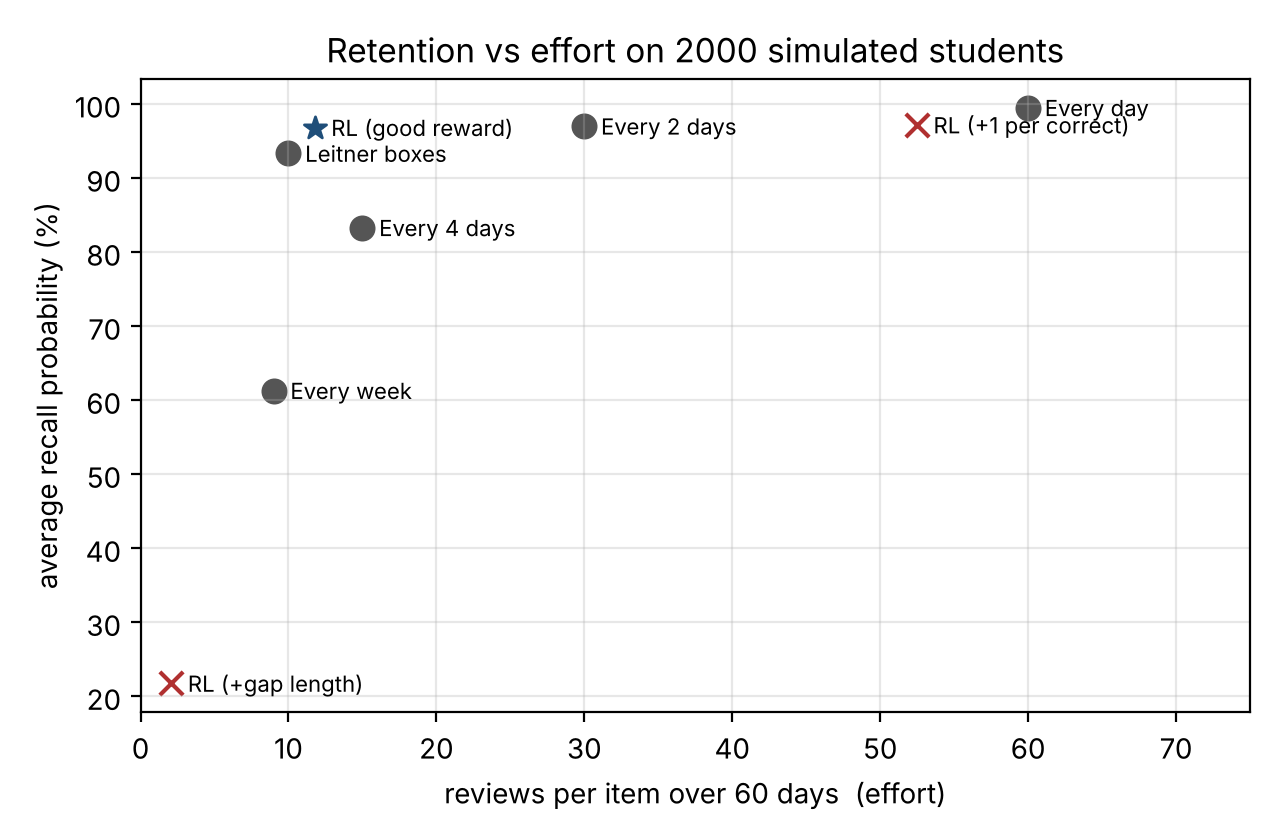
\includegraphics[width=0.8\linewidth]{benchmark.png}
\caption{Top-left is best: high recall, little effort. Red crosses are agents trained on bad rewards (next section).}\end{figure}

\subsection{What did the agent learn?}
\begin{center}
\begin{tabular}{@{}c|ccc@{}}
\textbf{streak} & \textbf{forgot} & \textbf{hard} & \textbf{easy}\\ \hline
0 & 1 & -- & --\\
1 & -- & 1 & 1\\
2 & -- & 1 & 1\\
3 & -- & 4 & 1\\
4 & -- & 1 & 4\\
5 & -- & 4 & 14\\
\end{tabular}
\end{center}
Next gap in days. Roughly: \emph{drill a new concept daily until it has a solid streak, then jump to long gaps.}
Some cells look odd (streak 3: hard $\rightarrow$ 4 days but easy $\rightarrow$ 1 day?). States that are visited rarely get few
updates --- a great discussion for the weekly meet, and the reason exercise 3 asks you to train with several seeds.

\bigsection{Reward hacking}{how a badly designed reward can make the agent ``cheat''.}
RL optimises \emph{exactly} what you reward, not what you meant. Two tempting rewards:
\begin{itemize}
  \item \textbf{+1 per correct answer.} Sounds right! The agent learns to quiz you almost every day
        (52.5 reviews per concept): easy points, huge workload. It games the metric.
  \item \textbf{+gap length} (``reward long gaps, they mean strong memory''). The agent simply never quizzes
        (2.1 reviews) and you keep \textbf{21.7\%} recall. It found the loophole: waiting is free.
\end{itemize}
This is not a toy problem: recommender systems that reward clicks learn clickbait; game agents find glitches.
\textbf{Designing the reward is the most important design decision you'll make in RL.}

\begin{task}{Week 4 assignment}
\begin{enumerate}[leftmargin=1.4em]
  \item Notebook exercises: Leitner 1 \& 3 (your own rule-based scheduler); RL 1, 3, 4 (review cost sweep, 5 seeds,
        invent a hackable reward).
  \item A \textbf{1-page comparison} (\texttt{starter/comparison.md}): your plot, your learned policy and what it means,
        one reward-hacking example, one limitation of the simulator.
\end{enumerate}
\end{task}

% ======================= WEEK 5 =======================
\weekbanner{Week 5}{RL Inside the Live Tutor}{Close the loop: the tutor quizzes you when the agent says so, Gemini
grades you, and every grade keeps training the agent while you study. Then: benchmark, demo, report.}

\bigsection{Architecture of Re-Mind 2.0}{everything you built, in one app.}
\begin{note}
\textbf{\texttt{app/streamlit\_app.py}} (UI) $\;\rightarrow\;$ \textbf{\texttt{remind/tutor.py}} (the agent) which uses
\textbf{\texttt{llm.py}} (Gemini: answer, extract concept, write quiz, grade) and
\textbf{\texttt{rl/qlearning.py}} (choose gap, learn from reward), and stores items in \textbf{\texttt{data/memory.json}}
and the Q-table in \textbf{\texttt{data/q\_table.json}}.
\end{note}
\subsection{One concept's life}
\begin{enumerate}[leftmargin=1.4em]
  \item You ask ``what is a Q-table?''. Gemini answers (directly or Socratically).
  \item \textbf{Concept extraction:} Gemini returns JSON \texttt{\{"topic": "Q-table", "fact": "..."\}}; the tutor stores an item
        with \texttt{streak=0}, \texttt{last\_grade=0}.
  \item \textbf{Scheduling:} the agent looks at state $(0, \text{forgot})$ and picks a gap, e.g.\ 1 day; \texttt{next\_due} is set.
  \item \textbf{Agency:} on every rerun the tutor checks \texttt{due\_items()}. When one is due it interrupts you with a quiz.
  \item \textbf{Grading:} Gemini returns \texttt{\{"grade": 0|1|2, "feedback"\}}.
  \item \textbf{Learning:} reward $= \pm$ actual days waited $- c$, exactly as in simulation; Q-update; new gap chosen.
\end{enumerate}

\subsection{From simulation to reality}
\begin{itemize}
  \item \textbf{Warm start.} A Q-table learned from scratch on one human would take months. So we pre-train on simulated
        students (\texttt{python scripts/train\_scheduler.py}) and \emph{fine-tune online} with a small $\varepsilon = 0.05$ ---
        the same idea as pre-training and fine-tuning LLMs.
  \item \textbf{Same state, same reward.} The live tutor uses the same 18 states and the same reward as the simulator,
        built from what it can observe: the streak, Gemini's grade, and the real time elapsed.
  \item \textbf{Time travel for demos.} Nobody waits 14 days for a demo. \texttt{REMIND\_DAY\_SECONDS=60} in \texttt{.env}
        makes one tutor-day last one minute.
  \item \textbf{Caveat.} Gemini's grade is a noisy measurement; the simulator is a cartoon of memory. Your report should
        discuss what could go wrong.
\end{itemize}

\subsection{Run it}
\begin{lstlisting}[style=shell]
python scripts/train_scheduler.py          # ~5 s, writes data/q_table.json
streamlit run app/streamlit_app.py
\end{lstlisting}
Ask 3--4 questions, wait a minute, and watch the tutor interrupt you. The sidebar lets you switch between Socratic
and direct mode and between the RL and Leitner schedulers.

\bigsection{End-Term submission}{Very Open ended, apply your own ideas !}
\begin{task}{Part A --- Core (required)}
Your own Re-Mind tutor (you may start from \texttt{app/streamlit\_app.py}) that (1) extracts and stores concepts in JSON,
(2) asks the pre-trained RL agent for the next gap, (3) quizzes on its own when an item is due, (4) grades with Gemini
(0/1/2, JSON) and uses the grade as reward to update the Q-table online, and (5) has a Socratic mode toggle.
\end{task}
\begin{task}{Part B --- At least one extension}
A bandit that learns which \emph{quiz style} works best for you $\cdot$ add difficulty/topic type to the RL state and
re-benchmark $\cdot$ a dashboard (recall curve per concept, Q-table heatmap, reward over time) $\cdot$ a function
approximator instead of a table $\cdot$ import an Anki/CSV deck $\cdot$ anything you can justify.
\end{task}
\begin{task}{Part C \& D --- Benchmark, demo and report}
Benchmark your scheduler against Leitner in simulation, record a $\le$ 3-minute demo, and write a $\le$ 4-page report
(\texttt{week5\_rl\_tutor/report\_template.md}): your design choices, your reward, results, one failure case, and one way
your reward could be hacked. Submit repo link + video + report PDF via the form.
\end{task}

% ======================= APPENDIX =======================
\appendix
\bigsection{Cheatsheet: RL notation}{pin this.}
\begin{center}
\renewcommand{\arraystretch}{1.25}
\begin{tabular}{@{}ll@{}}
\toprule
$s, a, r, s'$ & state, action, reward, next state\\
$\pi(s)$ & policy: action chosen in state $s$\\
$\gamma$ & discount factor (how much the future matters)\\
$\alpha$ & learning rate (step size)\\
$\varepsilon$ & exploration rate in $\varepsilon$-greedy\\
$G_t = \sum_k \gamma^k r_{t+k+1}$ & return\\
$Q(s,a)$ & expected return after taking $a$ in $s$\\
$Q \leftarrow Q + \alpha\,[r + \gamma\max_{a'} Q(s',a') - Q]$ & the Q-learning update\\
$P = 0.9^{t/S}$ & recall probability after $t$ days with stability $S$\\
\bottomrule
\end{tabular}
\end{center}

\bigsection{Resources}{for when you want more.}
\begin{itemize}
  \item Sutton \& Barto, \emph{Reinforcement Learning: An Introduction} (free online) --- ch.\ 2 (bandits) and 6 (Q-learning).
  \item David Silver's RL lectures (YouTube) --- lectures 1, 2 and 5.
  \item Gemini API docs: \url{https://ai.google.dev/gemini-api/docs}
  \item Streamlit chat apps tutorial: \url{https://docs.streamlit.io/develop/tutorials/chat-and-llm-apps}
  \item Open Spaced Repetition / FSRS: \url{https://github.com/open-spaced-repetition}
  \item Gwern, \emph{Spaced Repetition for Efficient Learning} --- the classic long read.
\end{itemize}

\end{document}
